\chapter{实验设置}
\label{chap:experiment}

我们利用大规模的真实数据集进行了实验,以定量评估所提出的算法框架。

\section{数据集}\label{sec:dataset}
我们的实验在微博的社交网络上进行。微博是中国最受欢迎的社交平台之一。
数据集来自网络爬虫\cite{Ren2014WeiboEvents},数据包含了微博id、微博作者id、微博发布时间以及评论数转发数等相当多的特征。完整的数据格式和各字段意义见附录。

使用tkipf-GCN框架\cite{kipf2017semi}还支持多个图实例(可能不同大小)的分批分类,每个实例都有一个邻接矩阵。最好是将各自的特征矩阵连接起来,并建立一个(稀疏)块对角矩阵,其中每个块对应于一个图实例的邻接矩阵。

这是模型的运行结果图,随着迭代次数的增加,过了500个epoch左右后,用训练数据测量到的识别精度几乎都为 100\%。但是,对于测试数据,离100\%的识别精度还有较大的差距。如此大的识别精度差距,是只拟合了训练数据的结果。出现了的过拟合现象(如图\ref{fig:epoch}),再经过正则化修正之后,选取迭代次数为200性能的GCN网络。
\begin{figure}[!htbp]
    \centering
    \begin{subfigure}[b]{0.35\textwidth}
      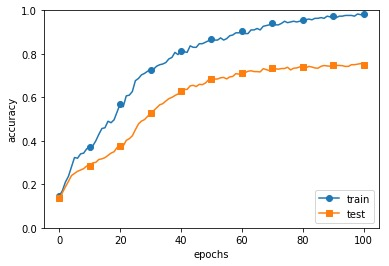
\includegraphics[width=\textwidth]{epoch100}
      \caption{}
      \label{fig:epoch100}
    \end{subfigure}%
    ~%add desired spacing
    \begin{subfigure}[b]{0.35\textwidth}
      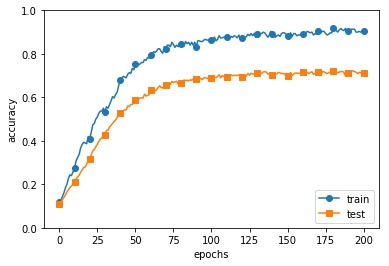
\includegraphics[width=\textwidth]{epoch200}
      \caption{}
      \label{fig:epoch200}
    \end{subfigure}%
    \begin{subfigure}[b]{0.35\textwidth}
      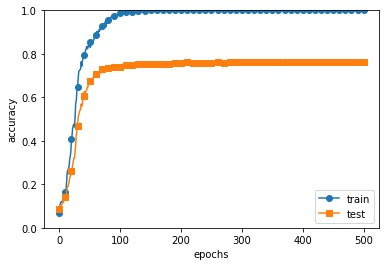
\includegraphics[width=\textwidth]{epoch500}
      \caption{}
      \label{fig:epoch500}
    \end{subfigure}%

    \caption{预测准确率,(a) 迭代次数为100次的GCN预测准确率,(b) 迭代次数为200次,(c) 迭代次数为500次。}
    \label{fig:epoch}
\end{figure}
该网络预测的准确率稳定在75\%左右,满足我们的实验要求。一份无特征缺失的数据保障了实验的进行。


这里,我们将处理过后的数据进行时间和空间尺度上的分析,下面是分析结果的可视化。
\begin{figure}[!htbp]
    \centering
    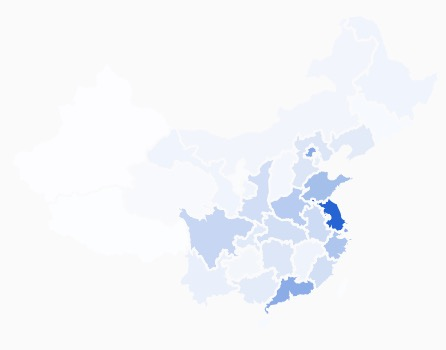
\includegraphics[width=0.50\textwidth]{Position}
    \caption{微博用户的地理分布}
    \label{fig:Position}
\end{figure}
图\ref{fig:Position}是微博用户的位置的可视化。从图\ref{fig:Position}中可以看出,该事件转发评论的微博用户主要集中在沿海地区,江苏尤为集中,内陆以四川、河南为代表,总体来说经济发达地区对此事件关注度普遍较高。因此,我们认为地理距离也是衡量社交相似性的一个重要特征。具体可以查看数据中省份城市编码,对照新浪微博的开发文档中的省份城市编码表。


时间尺度分析:
\begin{figure}[!htbp]
    \centering
    \begin{subfigure}[b]{0.5\textwidth}
      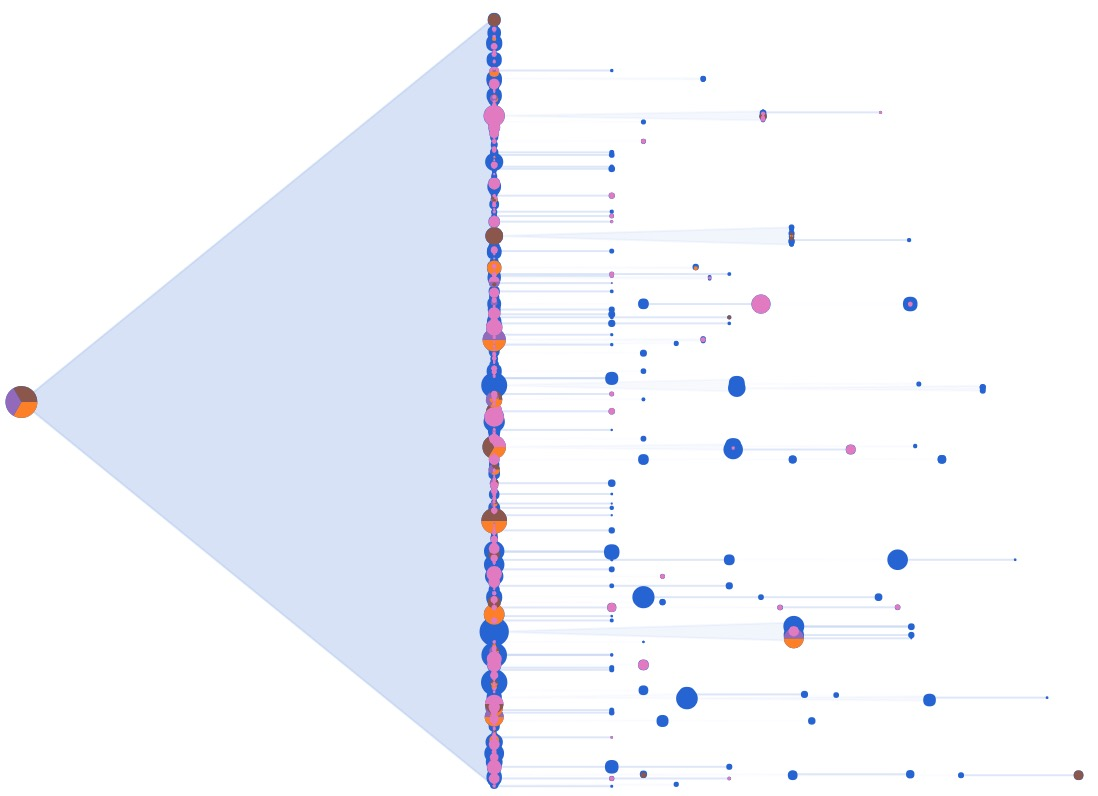
\includegraphics[width=\textwidth]{Tree}
      \caption{}
      \label{fig:Tree}
    \end{subfigure}%
    ~%add desired spacing
    \begin{subfigure}[b]{0.5\textwidth}
      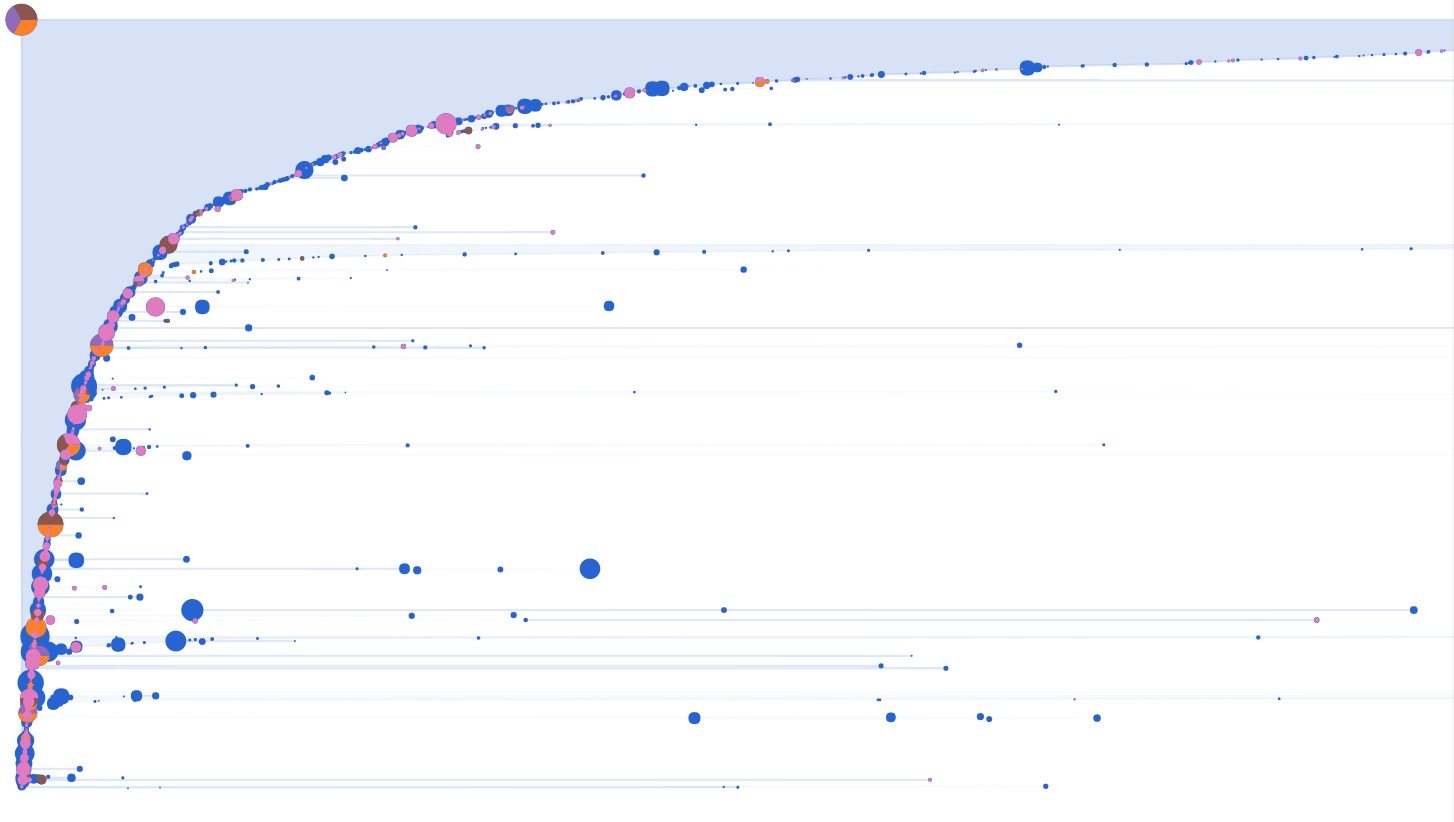
\includegraphics[width=\textwidth]{Sail}
      \caption{}
      \label{fig:Sail}
    \end{subfigure}%

    \caption{(a) 树形图,(b) 船帆图。}
    \label{fig:Time}
\end{figure}
如图\ref{fig:Time}所示。图\ref{fig:Tree}反映了各个转发层数随着时间的分布。通过观察我们可以发现,大多数意见领袖都处于第一层转发者,事件最多经过了7层转发。可见转发层数也是衡量一个事件影响力的重要特征。图\ref{fig:Sail}反映了各个转发节点随着时间的分布。



关键节点分析:如图\ref{fig:Repost}。图\ref{fig:Repost}中可以清楚地观察到事件的核心社交圈以及各个子社交圈的意见领袖及其分布。由此我们通过分析意见领袖的领域分布及其在各自领域的影响力来得出各个子社交圈的影响力。这些意见领袖在各自社交圈的影响力也成为了评估事件影响力的一个重要特征。
\begin{figure}[!htbp]
    \centering
    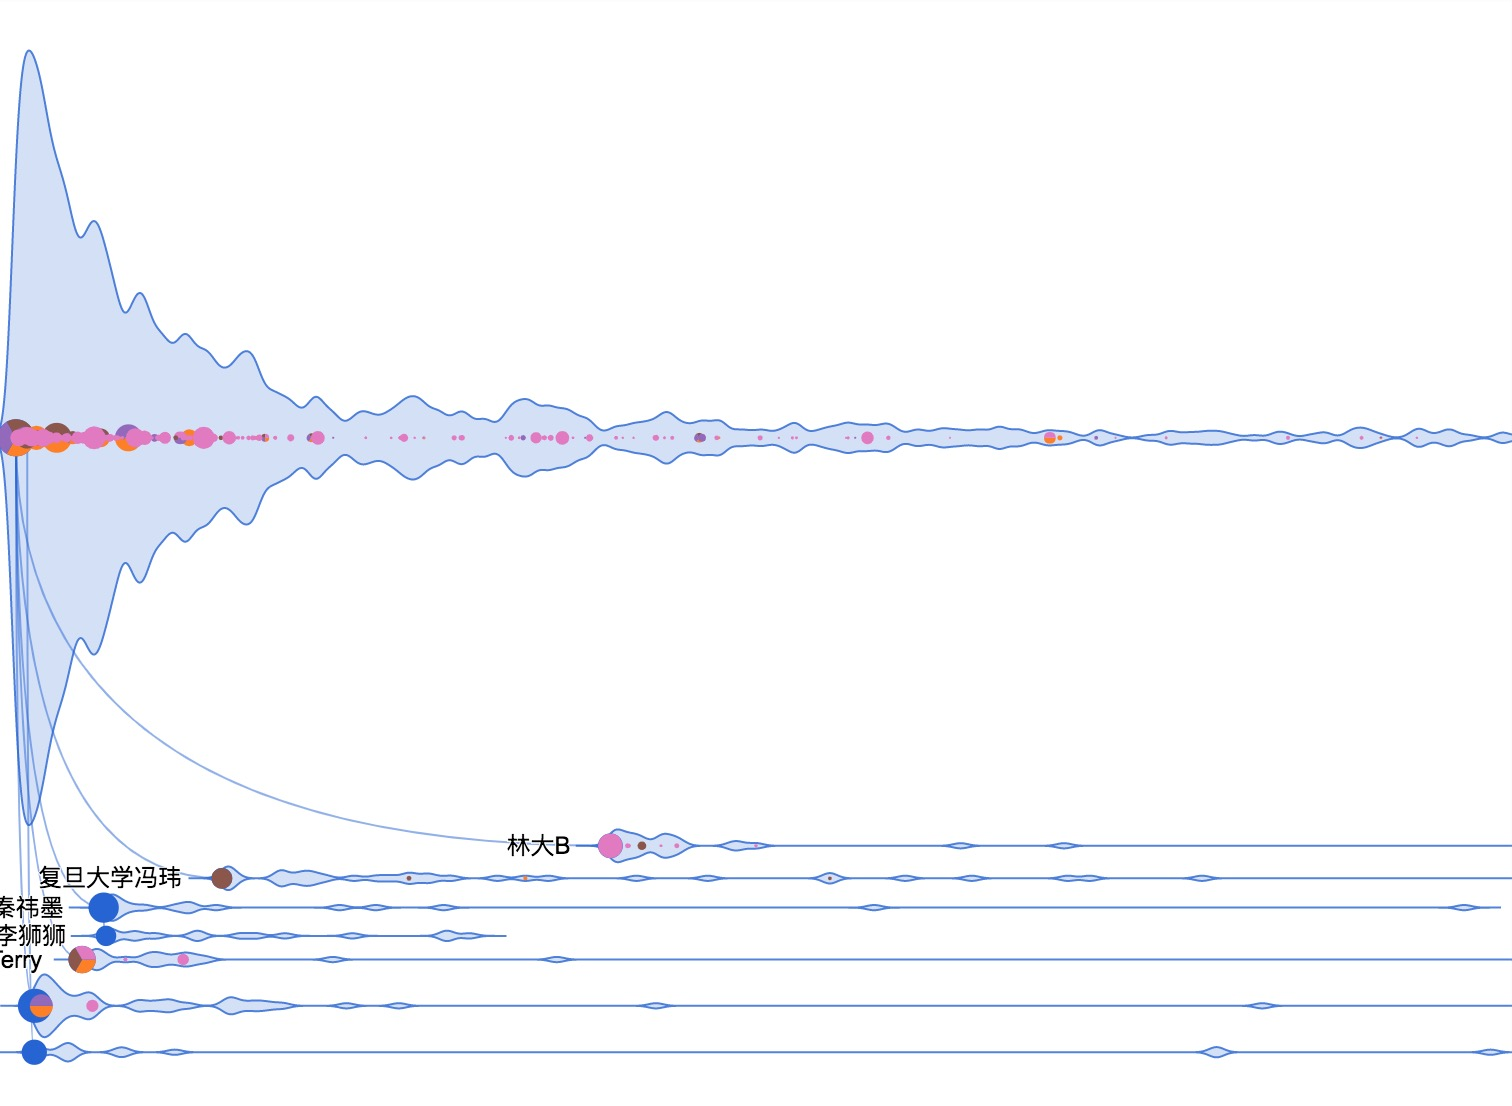
\includegraphics[width=0.5\textwidth]{Curves}
    \caption{话题热度随时间变化示意图}
    \label{fig:Curves}
\end{figure}
热度分析:




\section{评估指标}
为了定量评估本文的算法,我们使用以下性能指标:

预测性能~我们评估预测性能根据曲线下面积(AUC)、精度(Prec)、召回(Rec)和 F1 测量(F1)。

参数灵敏度~我们分析了我们的模型和测试不同的超参数选择如何影响预测性能。 

案例研究~我们使用具体案例来进一步证明和解释我们提出的算法的有效性。


\section{算法比较}

我们将GHSOM与几个算法进行比较。

逻辑回归(LR)使用逻辑回归(LR)来训练。该模型考虑了三类特征:(1)用户的顶点特征;(2)预训练网络嵌入;(3)手工制作的网络特征。

支持向量机(SVM)使用了支持向量模型。以线性核为分类模型的机器(SVM)。该模型使用与逻辑回归(LR)相同的特征。






